\section{Orientation: what problem does the paper solve?}
\label{sec:orientation}

Imagine that you manage a campaign for a new phone. You have weekly search volumes for a few
keywords in many countries. Three natural questions arise:

\begin{enumerate}
  \item \textbf{Where?} Which countries are most interested in each product?
  \item \textbf{From where to where?} If interest rises in the United States and rises a few
        weeks later in Vietnam, is that a sign of diffusion?
  \item \textbf{What next?} What will interest look like next week or next month in each place?
\end{enumerate}

D-Tracker is designed to answer these questions together on a \emph{tensor stream}, not merely
on a simple time-series table. Its central idea is not a large neural forecast. It is a small,
physically meaningful model that compresses the data while exposing the changing patterns.

\begin{keypoint}
D-Tracker decomposes observations into \textbf{trend + seasonal + outlier}. The trend is compressed
into a small core, and that core evolves under a \textbf{reaction--diffusion} system that represents
growth and spread across location groups. The model is updated as data arrive and switches to a
new model when the structure changes.
\end{keypoint}

\subsection{A small example with three kinds of signal}

Table~\ref{tab:running-example} is \textbf{an illustrative example created for this guide}, not a
result from the paper. Each cell is an interest index from 0 to 100.

\begin{table}[htbp]
  \centering
  \small
  \caption{Illustrative example: one keyword has different interest across locations and time.}
  \label{tab:running-example}
  \begin{tabular}{llrrr}
    \toprule
    Keyword & Location & Week 1 & Week 2 & Week 3 \\
    \midrule
    iPhone & United States & 80 & 84 & 90 \\
    iPhone & Vietnam & 15 & 22 & 35 \\
    Galaxy & United States & 45 & 40 & 32 \\
    Galaxy & Vietnam & 30 & 34 & 40 \\
    \bottomrule
  \end{tabular}
\end{table}

At least three things are happening. First, ``iPhone'' rises in both places, but more strongly in
the United States. Second, the rise in Vietnam follows the United States in this example --- a
\emph{candidate} for interest diffusion, not evidence of causation. Third, ``Galaxy'' falls in the
United States while rising in Vietnam, so the trend is not the same for every keyword--location
pair. Real data also contain seasonality (product launches, year-end sales) and sudden spikes.

\begin{plainwords}
Looking at one line makes it easy to confuse seasonality with trend and a one-off spike with
diffusion. D-Tracker first separates the three sources of signal, then looks for structure in the
trend part.
\end{plainwords}

\subsection{Three challenges and three promises}

The paper emphasizes three difficulties. The data have \textbf{complex patterns} (trend,
seasonality, diffusion, outliers); those patterns \textbf{change over time}; and the data form a
high-dimensional tensor that is \textbf{semi-infinite} in time. The authors summarize their answer
with three properties in the introduction and conclusion:

\begin{description}[leftmargin=1.8em,style=nextline]
  \item[Interpretable.] The latent core and non-negative factors show which location/keyword groups
  relate to each dynamics and in which direction interest spreads. This is interpretability
  \emph{through model structure}, not a proof of causal effects.
  \item[Automatic.] The latent dimensions and model-switch times are selected with a compression
  criterion (MDL), rather than asking a user to try configurations by hand. Numerical optimizers
  still have settings; the user does not manually choose ``two groups or three?'' for each period.
  \item[Scalable.] Each update processes only a fixed-length recent window, so runtime does not grow
  with the total length of the stream. The paper reports being up to 8.0$\times$ faster and ``up to
  57\% improvement'' than competitors. The 57\% sentence names neither the metric nor its
  denominator, so these are paper claims, not a normalized effect size or a reproduction in this repo.
\end{description}

\begin{commonmistake}
``Scalable'' here does not mean that every operation is $O(1)$. It means that processing one stream
step does not depend on how long the stream has already become, because only a window is retained.
Cost still grows with the number of keywords, locations, and latent dimensions.
\end{commonmistake}

\subsection{See the result before learning the machinery}

\begin{figure}[htbp]
  \centering
  \begin{subfigure}[t]{0.92\linewidth}
    \centering
    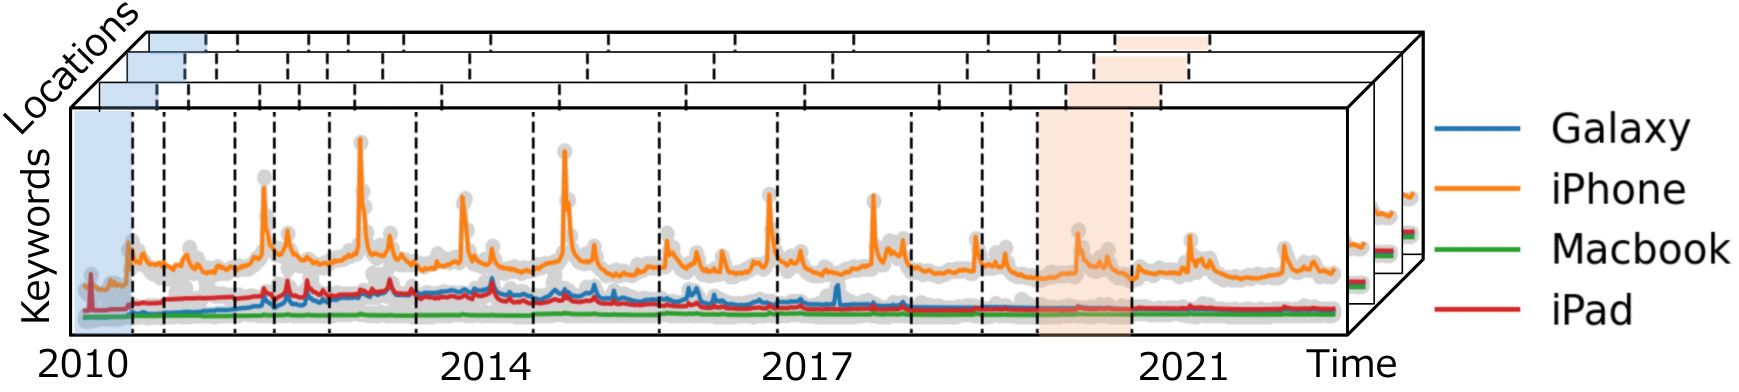
\includegraphics[width=\linewidth]{figures/Figure1_a.png}
    \caption{Observations (gray) and model fit (color); dotted vertical lines mark model switches.}
  \end{subfigure}

  \vspace{4mm}
  \begin{subfigure}[t]{0.82\linewidth}
    \centering
    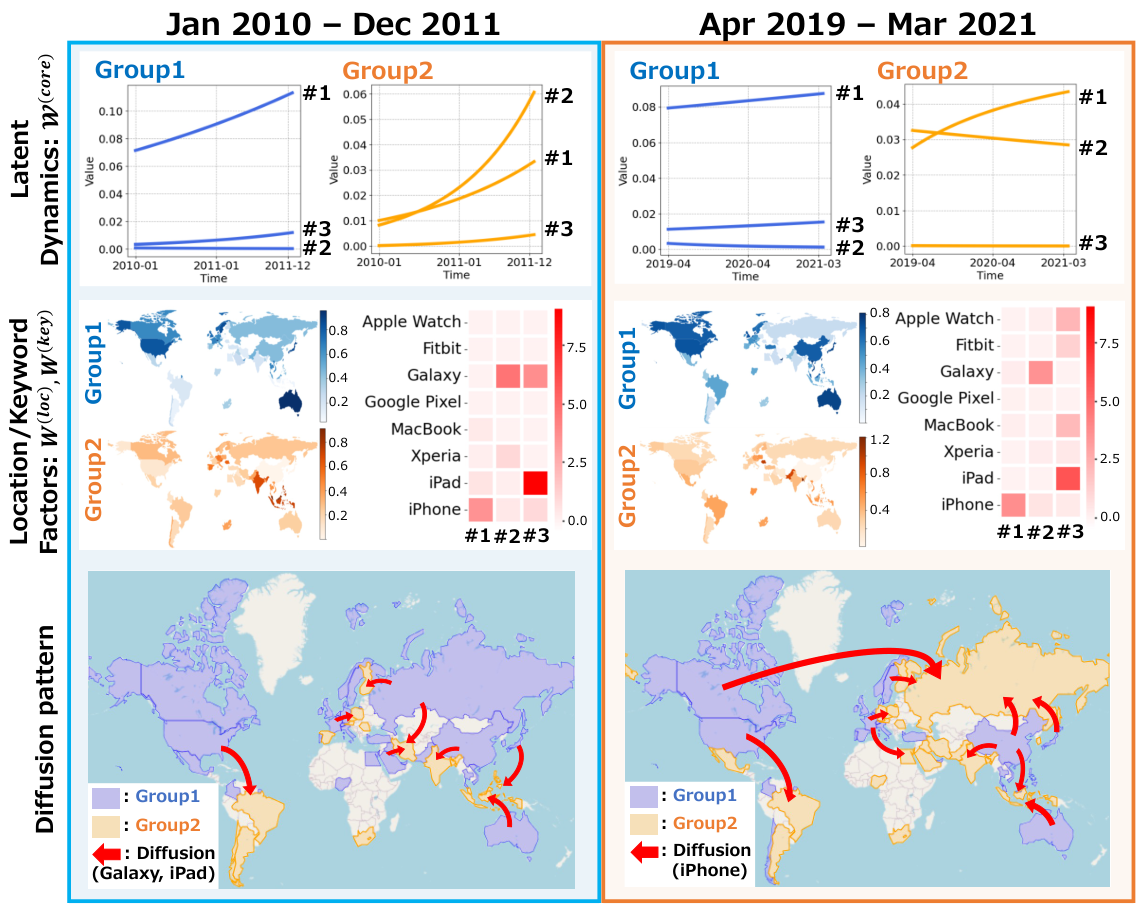
\includegraphics[width=\linewidth]{figures/Figure1_b.png}
    \caption{Latent dynamics, location/keyword factors, and diffusion maps in two periods.}
  \end{subfigure}
  \caption{Modeling power of D-Tracker on the device data. Source: Higashiguchi et al. (2025),
  arXiv:2505.00242v1, Figure~1; author-owned figure, CC BY 4.0.}
  \label{fig:preview}
\end{figure}

In Figure~\ref{fig:preview}(a), the model does not use one parameter set for the whole displayed period. The
dotted lines split the stream into periods, each modeled separately. This is \emph{regime switching}.
In Figure~\ref{fig:preview}(b), each column is one dynamics: the top curve is the core
$\mathcal{W}^{(\mathrm{core})}$ over time; the middle row shows how strongly that dynamics relates
to keywords and location groups; the bottom row shows diffusion arrows between groups. We therefore
get more than a forecast: a testable story about which dynamics, keyword, region, and direction.

\begin{figure}[htbp]
  \centering
  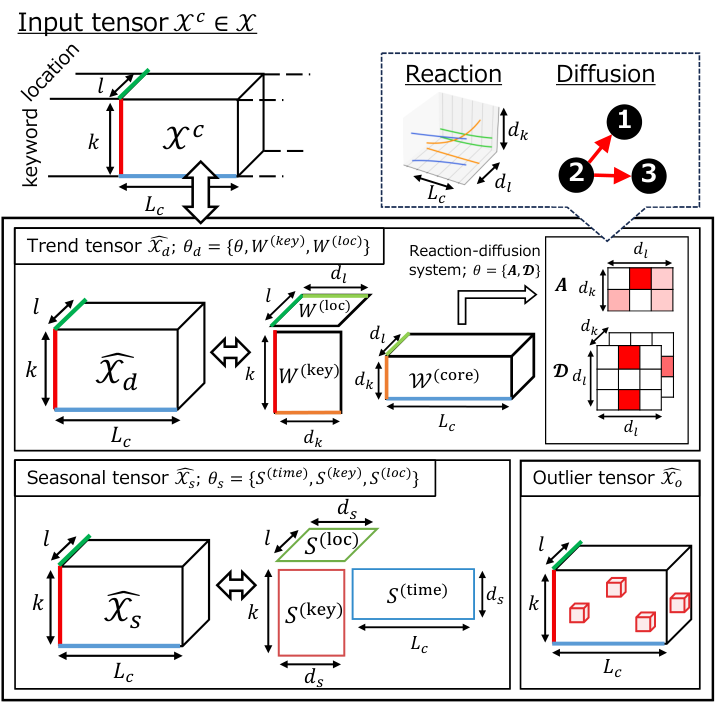
\includegraphics[width=0.72\linewidth]{figures/overview.png}
  \caption{D-Tracker overview: the current tensor is approximated by trend + seasonal + outlier.
  Source: Higashiguchi et al. (2025), arXiv:2505.00242v1, Figure~2; author-owned figure, CC BY 4.0.}
  \label{fig:overview}
\end{figure}

Figure~\ref{fig:overview} is the map of the whole paper. The input is the current tensor
$\mathcal{X}^{c}$. Its three branches encode three assumptions: a slowly changing/spreading part, a
periodic part, and a sparse unusual part. Section~\ref{sec:model} explains why the trend is
compressed into a small core and why that core can be generated by differential equations.

\begin{selfcheck}
\begin{enumerate}
  \item Why can a single model for the entire stream fail even when a lot of history is available?
  \item Which of the three questions at the start of the chapter do trend, seasonal, and outlier address?
  \item What model structure makes D-Tracker interpretable, and what does that interpretation \emph{not} claim?
\end{enumerate}
\end{selfcheck}
